% Sample file on how to use subfiles.
\documentclass[micro_gen.tex]{subfiles}

\begin{document}

\chapter{Microstructure generation}

\textbf{A bit more here about why use of Voronoi, analytical, approximates grain size distribution etc...}

A Voronoi tessellation is a partition of a domain $D \in \mathbb{R}^d$ into $n$ regions $R_i$ in $D$, each corresponding to one of $n$ different \textit{seed points} $\vec{P}_i$. These regions consists of the set of all points that are closer to a particular seed point than to any other,
%
\[R_i = \{ \vec{x} \in D : \left|\left| \vec{P}_i - \vec{x} \right|\right| < \left|\left| \vec{P}_j - \vec{x} \right|\right| \quad  \forall i \neq j, \quad i,j = 1, \ldots, n \}. \]
%
In this thesis the norm used is the Euclidean distance, the dimension of the space is 3 and the bounding domain is a cube. In this case, the resulting regions will have the shape of convex polyhedrons which is referred to as \textit{grains}. Two grains will intersect over a plane called a \textit{face}, three along a line called an \textit{edge} and four will intersect in a point called a \textit{vertex}.
A common way to set the locations of the seed points is to randomly assign them to different positions in $D$. This is known as a "Poisson-Voronoi tesselation". An example of such a tessellation can be seen in figure \ref{fig:pois_voronoi} where 100 seed points have been used.

The generation of the tessellation can easily be done in for example the commonly used software MATLAB \cite{matlab:voronoi}. In this thesis the open source software Neper \cite{Quey20111729} was used to generate the tessellation since this software is also capable of meshing the generated structure. 




\begin{figure}
\centering
\begin{subfigure}[b]{.5\textwidth}
  \centering
  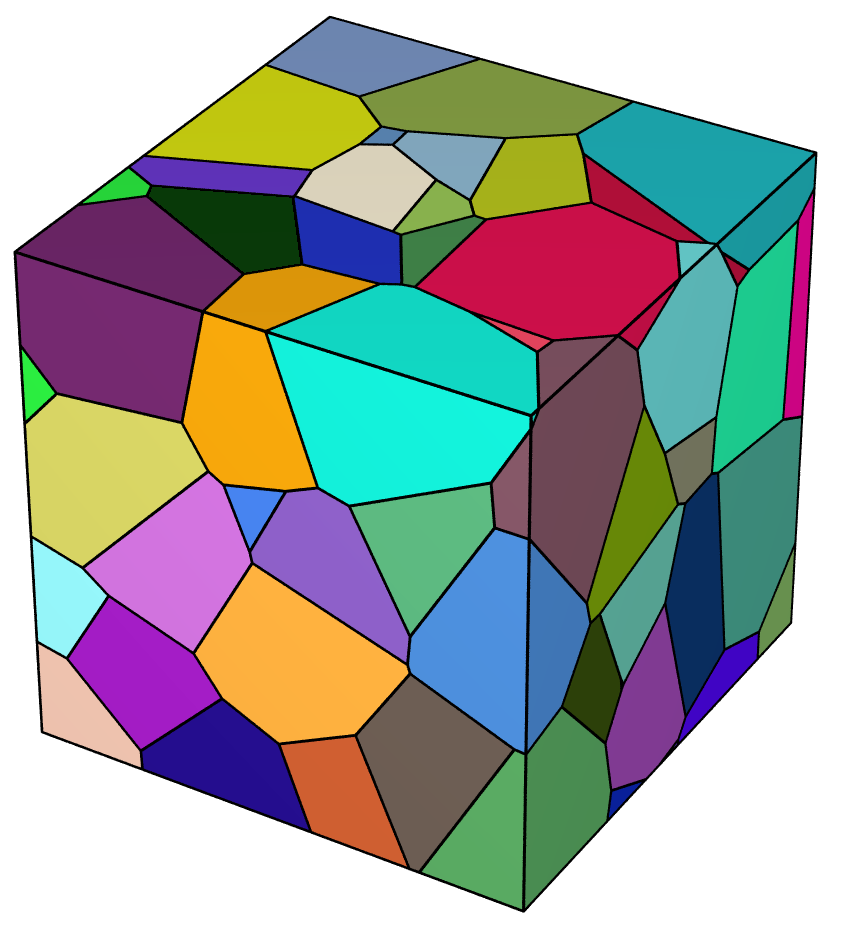
\includegraphics[width=.5\linewidth]{./figures/img_body.png}
  \caption{All polyhedrons shown.}
  \label{fig:pois_voronoi_a}
\end{subfigure}%
\begin{subfigure}[b]{.5\textwidth}
  \centering
  \includegraphics[width=.5\linewidth]{./figures/img_nobody.png}
  \caption{Polyhedrons that are part of the domain boundary hidden.}
  \label{fig:pois_voronoi_b}
\end{subfigure}
\caption{Voronoi tessellation containing 100 polyhedrons bounded by a cube}
\label{fig:pois_voronoi}
\end{figure}



\end{document}
